
\fullcite{thkp15}

\begin{multicols}{2}
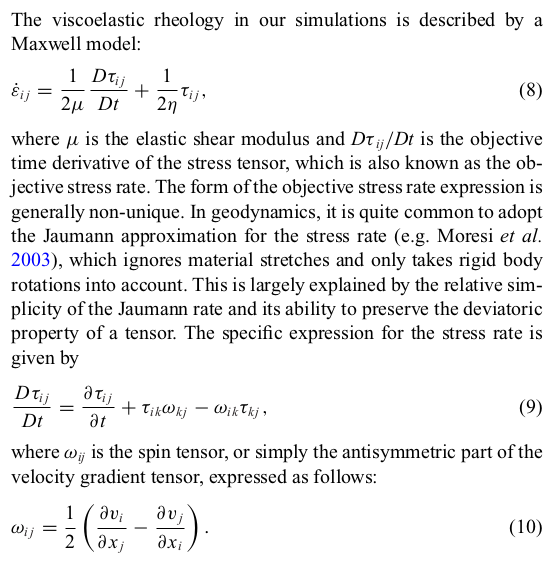
\includegraphics[width=8.25cm]{images/viscoelasticity/thkp15a}\\
\[
\dot{\bm\varepsilon} = 
\frac{1}{2\mu} \frac{{\cal D}{\bm \tau}}{{\cal D}t}
+\frac{1}{2\eta} {\bm \tau}
\]
Is is dev stress or full stress !?
\[
\frac{{\cal D} {\bm \tau}}{{\cal D}t} = 
\frac{\partial {\bm \tau}}{\partial t}  
+ {\bm \tau} \cdot \dot{\bm\omega} 
- \dot{\bm\omega} \cdot {\bm \tau}
\]
\end{multicols}

\begin{multicols}{2}
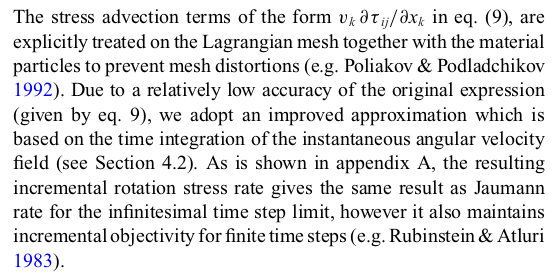
\includegraphics[width=8.25cm]{images/viscoelasticity/thkp15b}
\end{multicols}

\begin{multicols}{2}
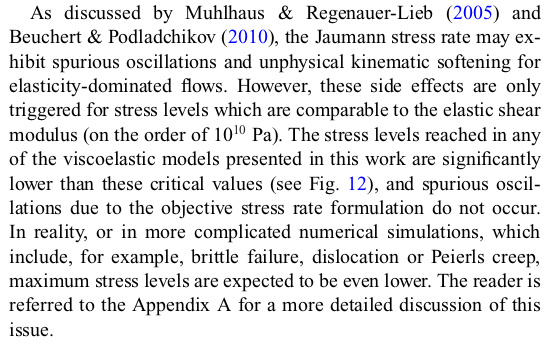
\includegraphics[width=8.25cm]{images/viscoelasticity/thkp15c}
\end{multicols}

\newpage
\paragraph{Discretization and solution}.

\begin{multicols}{2}
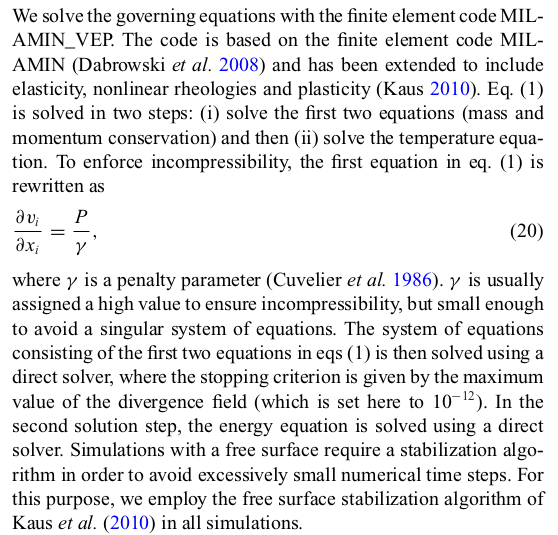
\includegraphics[width=8.25cm]{images/viscoelasticity/thkp15d}\\
\[
\vec\nabla\cdot \vec\upnu = \frac{1}{\lambda}p
\]
where $\lambda$ is a penalty parameter!
\end{multicols}

\begin{multicols}{2}
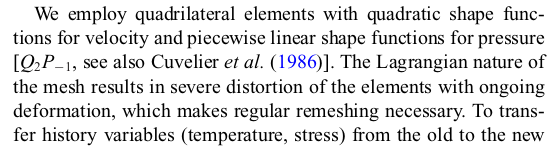
\includegraphics[width=8.25cm]{images/viscoelasticity/thkp15e}\\
$Q_2 \times P_{-1}$ element, discontinuous pressure field.
\end{multicols}

\begin{multicols}{2}
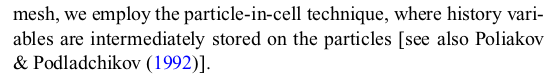
\includegraphics[width=8.25cm]{images/viscoelasticity/thkp15f}
\end{multicols}

\paragraph{Numerical formulation of viscoelasticity}.

\begin{multicols}{2}
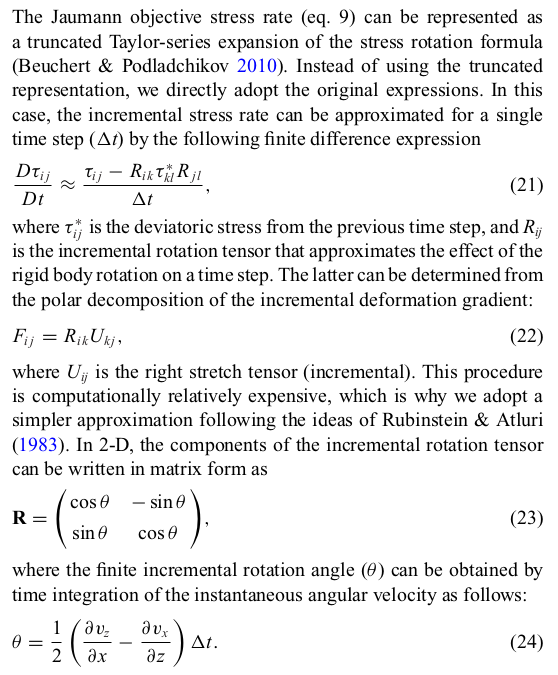
\includegraphics[width=8.25cm]{images/viscoelasticity/thkp15g}\\
\[
\frac{D \tau_{ij}^{k+1}}{Dt} \simeq \frac{\tau_{ij}^{k+1}- R_{ik}  \tau_{kl}^k R_{jl} }{\delta t}
\]
\[
{\bm R} = \left(\begin{array}{cc}
\cos\theta & -\sin \theta \\
\sin\theta & \cos\theta
\end{array}\right)
\]
\[
\theta = \frac12 \left(\frac{\partial v_z}{\partial x} - \frac{\partial v_x}{\partial z} \right) \delta t
\]
\end{multicols}

\begin{multicols}{2}
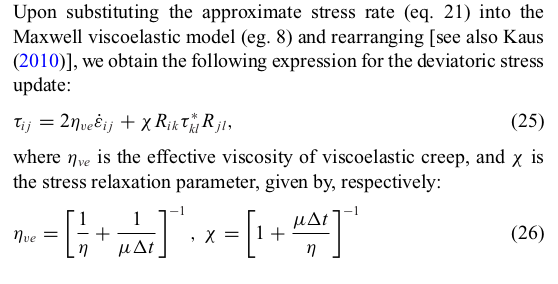
\includegraphics[width=8.25cm]{images/viscoelasticity/thkp15h}\\
\[
{\bm\tau}_{ij}^{k+1} = 2 \eta_{ve} \dot{\varepsilon}_{ij} + \xi R_{ik}  \tau_{kl}^k R_{jl} 
\]
with 
\[
\eta_{ve} = 
\left(
\frac{1}{\eta} + \frac{1}{\mu \delta t}
\right)^{-1}
\qquad
\xi = 
\left(
1 + \frac{\mu\delta t}{\eta}
\right)^{-1}
\]
\end{multicols}









